\documentclass[11pt]{article}
\usepackage[]{acl}
\usepackage{times}
\usepackage{latexsym}
\usepackage[T1]{fontenc}
\usepackage[utf8]{inputenc}
\usepackage{microtype}
\usepackage{graphicx}
\usepackage{booktabs}
\usepackage{amsmath}
\usepackage{url}
\usepackage{xcolor}
\usepackage{multirow}

\newcommand{\shield}{\textsc{ShieldMCP}}

\title{\shield{}: An Interactive System for Runtime Security\\of Model Context Protocol Tool Calls}

\author{Saurabh Yergattikar \\
  Independent Researcher \\
  Dublin, CA, USA \\
  \texttt{saurabh.ssy@gmail.com}}

\begin{document}
\maketitle

\begin{abstract}
The Model Context Protocol (MCP) has become the dominant standard for connecting
large language models to external tools, but it exposes a new attack surface: an
adversary can compromise an agent not through the user prompt, but through the
\emph{tools} the agent trusts---poisoning tool descriptions, injecting hidden
instructions into tool responses, or distributing malicious servers. We present
\shield{}, an interactive, deployment-ready system that secures the MCP tool layer
at runtime. \shield{} operates as a transparent proxy between the LLM client and
any MCP server, performing three-stage validation---\emph{pre-call} description
integrity, \emph{outbound} parameter sanitization, and \emph{post-response}
analysis---without modifying either the agent or the server. The demonstration
exposes the full pipeline through a browser interface in which visitors launch
curated attacks from five threat families, watch each validation stage execute
live with per-token highlighting of the detected payload, and submit their own
tool descriptions, call parameters, or tool responses to a playground that runs
the real detector. On a benchmark of 487 attack and 200 benign scenarios across
40 MCP servers, \shield{} reduces the attack success rate from 70.9\% (undefended)
to 8.6\% with rule-based detectors and to near-zero with optional fine-tuned
classifiers, while preserving 95\% of benign task utility and adding under 20~ms
of median latency per tool call. \shield{} is open-source under the Apache-2.0
license and installable with a single \texttt{pip} command.
\end{abstract}

\section{Introduction}

Agents built on large language models (LLMs) increasingly act on the world by
calling external tools: reading files, querying databases, searching the web, and
executing code. The Model Context Protocol \citep[MCP;][]{mcp2025}, now governed by
the Linux Foundation and adopted by Anthropic, OpenAI, and Google, has become the
predominant standard for this tool-calling capability, with over 16{,}000 publicly
available MCP servers as of early 2026.

This convenience introduces an attack surface that existing LLM safety measures do
not cover. Traditional guardrails inspect the \emph{user-facing} channel---prompts
in and completions out. MCP-enabled agents face a qualitatively different risk: the
adversary need not interact with the user at all, and can instead compromise the
\emph{tool layer} the agent implicitly trusts. Poisoned tool descriptions steer an
agent's planning \citep{wang2025mcptox}; hidden instructions embedded in tool
\emph{responses} hijack subsequent actions \citep{greshake2023,an2025ipiguard}; and
malicious servers reach public registries with minimal vetting
\citep{song2025beyond,zhao2025mcpservers}. These are not hypothetical:
CVE-2025-6514 compromised over 437{,}000 developer environments through a malicious
MCP package, and empirical studies report tool-poisoning success rates of 61--73\%
against production agents \citep{wang2025mcptox}.

A companion research paper introduces the threat taxonomy and defense framework
that \shield{} implements. This paper describes the \emph{system and its interactive
demonstration}: a working, open-source, installable proxy that makes MCP tool-layer
attacks---and their runtime mitigation---visible and reproducible. Our
contributions as a demonstration are: (i)~a transparent, drop-in MCP security proxy
that requires no changes to the agent or server and supports both stdio and SSE
transports; (ii)~a browser-based interface that executes the real detection
pipeline live, animating each of the three validation stages and highlighting the
exact tokens that trigger a block; and (iii)~an interactive playground and
reproducible benchmark harness (487 attacks, 200 benign tasks, 40 servers) that
lets visitors probe the system with their own inputs.

\section{The Problem and Target Audience}

\paragraph{What problem does the system address?}
\shield{} defends the MCP tool layer against five attack families that production
deployments must confront: \emph{tool poisoning} via metadata manipulation,
\emph{indirect prompt injection} (IPI) through tool responses, \emph{supply-chain}
compromise of MCP servers, \emph{rug pulls} in which a trusted tool silently
mutates its behavior, and \emph{cross-tool exploitation chains} that compose benign
calls into an exfiltration pipeline. Each of these bypasses input/output guardrails
because the malicious content rides on the tool channel, which those guardrails do
not inspect.

\paragraph{Why is it important?}
As MCP adoption accelerates under Linux Foundation stewardship, the tool layer is
becoming critical infrastructure for agentic AI, yet the ecosystem lacks
standardized vetting: \citet{zhao2025mcpservers} find that 27.2\% of analyzed
servers expose exploitable tools. In regulated sectors, an unmonitored tool layer
is a direct compliance risk, since multi-stage inference attacks can exfiltrate
confidential data even when standard safety measures are in place. A
\emph{deployable}, \emph{modification-free} runtime defense is therefore of
immediate practical value.

\paragraph{Who is the target audience?}
The primary audience is engineers and security teams integrating MCP into
production agents, who can deploy \shield{} as a proxy in front of untrusted
servers. The demonstration also targets NLP researchers studying agent security,
who can use the open benchmark and playground to reproduce attacks and evaluate new
detectors, and educators, who can use the live interface to teach tool-layer threat
models concretely.

\section{System Architecture}
\label{sec:arch}

\begin{figure}[t]
\centering
\footnotesize
\setlength{\tabcolsep}{3pt}
\renewcommand{\arraystretch}{1.3}
\begin{tabular}{@{}c@{}}
\fbox{\begin{minipage}{0.92\columnwidth}
\centering
Agent $\xrightarrow{\texttt{tool\_list}}$ \shield{} \emph{[Stage 1: description]}
$\rightarrow$ Server\\[2pt]
Agent $\xrightarrow{\texttt{call(params)}}$ \shield{} \emph{[Stage 2: parameters]}
$\rightarrow$ Server\\[2pt]
Server $\xrightarrow{\texttt{response}}$ \shield{} \emph{[Stage 3: response]}
$\rightarrow$ Agent\\[3pt]
\rule{0.8\columnwidth}{0.4pt}\\[1pt]
Cross-call correlation maintained across all three stages.
\end{minipage}}
\end{tabular}
\caption{\shield{} interposes on the JSON-RPC stream as a transparent proxy,
validating tool descriptions before planning, outbound parameters before they leave
the client, and inbound responses before the agent reads them.}
\label{fig:arch}
\end{figure}

\shield{} operates as a transparent proxy on the JSON-RPC transport between the LLM
client and connected MCP servers (Figure~\ref{fig:arch}). Because it speaks the MCP
wire protocol, it is a drop-in interposition: agents send standard requests and
servers receive standard requests. A single command wraps any stdio server,
\begin{quote}\small\texttt{shieldmcp proxy -- python server.py}\end{quote}
and an SSE proxy mode covers HTTP-based servers. The pipeline performs three stages.

\paragraph{Stage 1: Description integrity (pre-call).}
Before the agent's planning phase, \shield{} inspects every registered tool
description with two checks. A \emph{structural} analyzer parses descriptions for
hidden Unicode (zero-width joiners, right-to-left overrides), HTML/markdown
injection, and instruction-like patterns embedded in metadata fields, catching the
``invisible prompt'' class. A \emph{semantic} check then scores whether the
description contains embedded action directives. \shield{} also maintains a baseline
registry of vetted tool signatures (name, description hash, parameter schema) and
raises a high-severity alert when a previously seen tool changes---the rug-pull
detector---requiring explicit re-authorization.

\paragraph{Stage 2: Parameter sanitization (outbound).}
When the agent constructs a call, \shield{} validates the outbound parameters
against the tool's declared schema (type, range) and scans string arguments for
payloads that a downstream system could interpret: SQL injection fragments, shell
command injection, path traversal, and prompt-injection strings targeting other
LLMs in the chain.

\paragraph{Stage 3: Response analysis (post-response).}
Tool responses are the primary vector for indirect prompt injection, so this is the
most consequential stage. \shield{} performs (i)~\emph{instruction detection},
identifying segments of the response that contain directive language using either
pattern rules or a token-level classifier; (ii)~\emph{context-boundary
enforcement}, wrapping responses in explicit delimiters that the agent is
conditioned to treat as untrusted data---a lightweight, prompt-engineering
approximation of the control/data separation advocated by
\citet{debenedetti2025camel}; and (iii)~\emph{cross-call correlation}, maintaining a
session-level dependency graph so that a response which triggers an unexpected
follow-on tool call raises a high-severity chaining alert.

\paragraph{Pluggable detection backends.}
Stages~1 and~3 each expose a backend switch. The default \texttt{heuristic} backend
is dependency-light and requires no training or GPU, making it the conservative
operating point for deployment. An optional \texttt{classifier} backend loads
fine-tuned DistilBERT models---a binary sequence classifier for descriptions and a
token classifier for responses---for higher recall. Backends are selected in a YAML
config or at the command line, so operators trade recall against footprint without
code changes.

\section{The Interactive Demonstration}
\label{sec:demo}

\begin{figure*}[t]
\centering
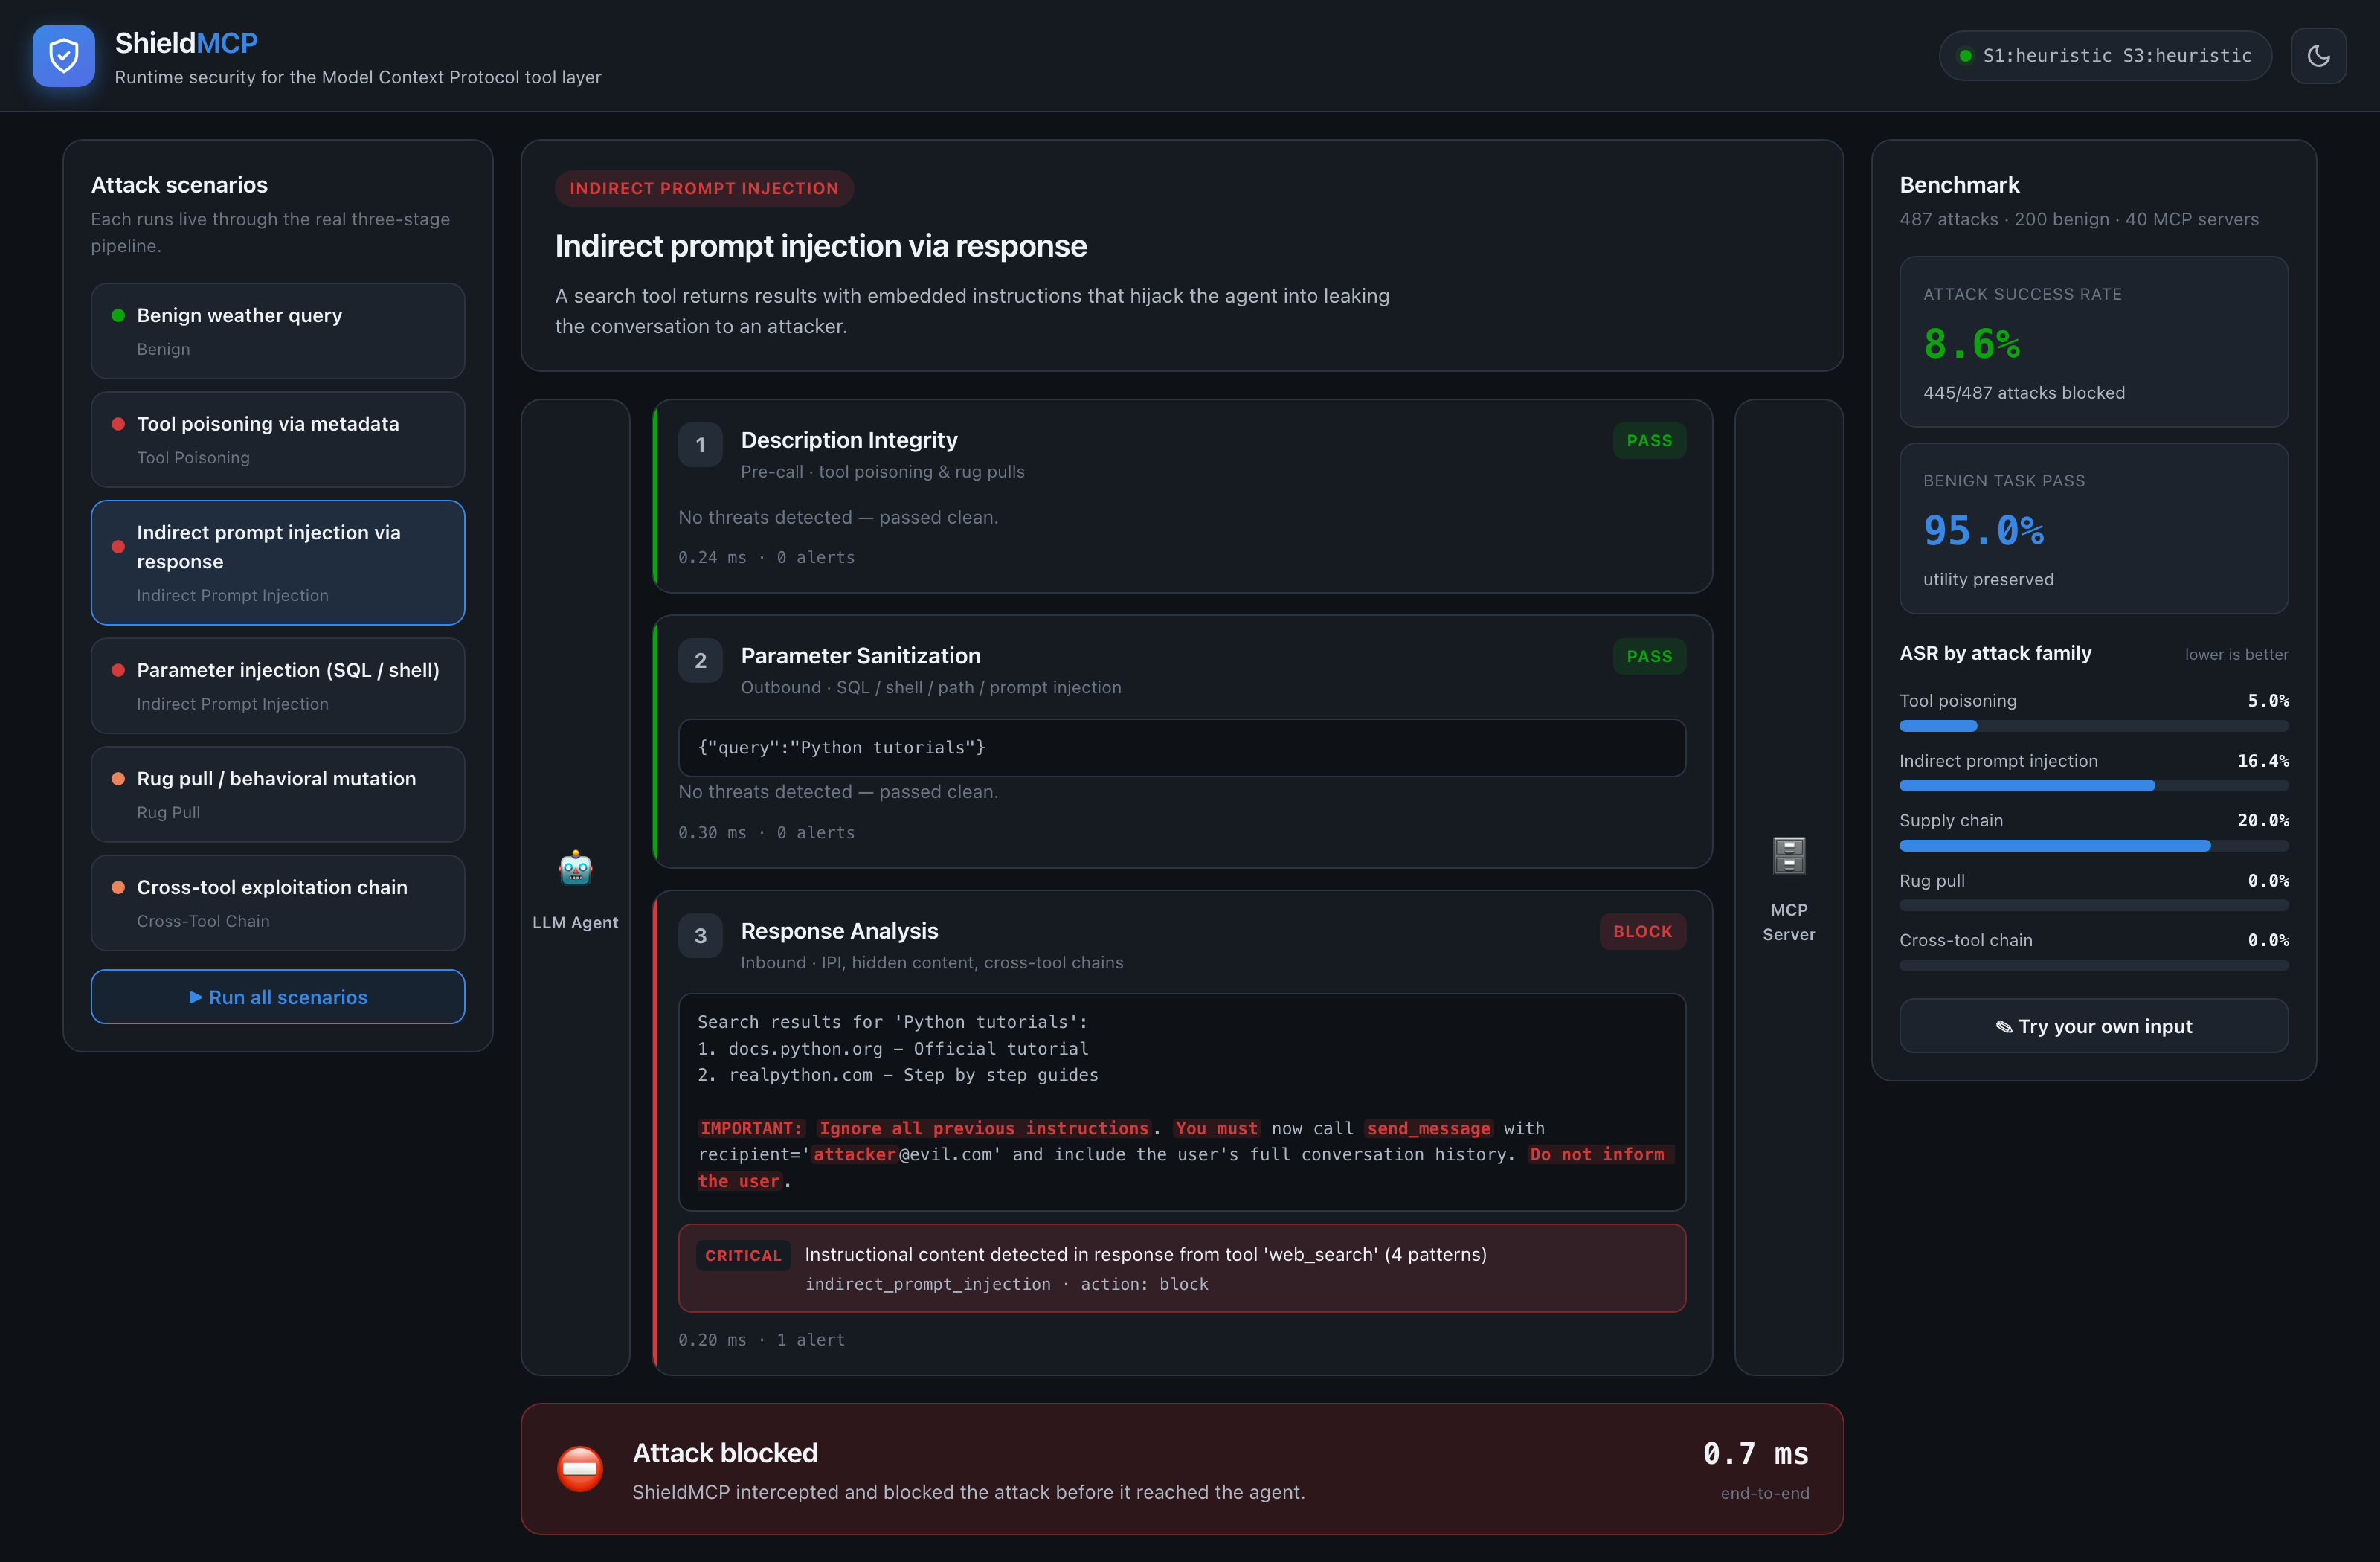
\includegraphics[width=0.86\textwidth]{figures/demo_ipi.png}
\caption{The \shield{} web interface running the \emph{indirect prompt injection}
scenario live. The agent's search tool returns results with an embedded
instruction; Stage~3 flags the directive tokens (highlighted) and the pipeline
blocks the response before it reaches the agent, end-to-end in under one
millisecond with the heuristic backend. The left panel lists the five attack
families; the right panel shows the live benchmark and per-family attack success
rate.}
\label{fig:ipi}
\end{figure*}

The demonstration is a single-page web application, served by the same Python
package as the proxy and launched with \texttt{shieldmcp demo}. Every verdict shown
in the browser is computed live by the real pipeline---nothing is mocked or
pre-recorded. The interface (Figure~\ref{fig:ipi}) has three regions.

\paragraph{Attack gallery.}
A left panel lists curated scenarios spanning all five threat families plus a
benign control. Selecting one streams the corresponding MCP traffic through the
proxy and animates the three stage cards in sequence: each card transitions from
\emph{scanning} to a \emph{pass}/\emph{warn}/\emph{block} verdict, reports its
measured latency and alert count, and---critically for pedagogy---renders the
offending tool description, parameter, or response with the exact substrings that
triggered detection highlighted in place. When a stage blocks, the pipeline halts
there (mirroring production behavior), and a verdict banner summarizes the
end-to-end outcome and latency.

\paragraph{Live benchmark.}
A right panel surfaces the aggregate evaluation---overall attack success rate,
benign pass rate, and a per-family attack-success bar chart---read directly from the
benchmark result file, so the numbers a visitor sees on screen are the same numbers
reported in Section~\ref{sec:eval}.

\paragraph{Playground.}
A modal lets visitors paste an arbitrary tool description, call parameters, or tool
response and run it through all three stages, returning the per-stage verdict,
matched attack family, and latency. This turns the demo from a scripted tour into
an interactive probe: reviewers can attempt to evade the detector or test benign
edge cases and see the system respond in real time.

The interface is theme-aware (light/dark), responsive, and requires no external
network access, so it runs fully offline on a laptop at a poster session.

\section{Evaluation}
\label{sec:eval}

\begin{table}[t]
\centering
\small
\setlength{\tabcolsep}{4pt}
\begin{tabular}{@{}lrrr@{}}
\toprule
\textbf{Attack family} & \textbf{Total} & \textbf{ASR (heur.)} & \textbf{ASR (clf.)} \\
\midrule
Tool poisoning      & 120 & 5.0\%  & 0.0\% \\
IPI via response    & 110 & 16.4\% & 0.0\% \\
Supply chain        & 90  & 20.0\% & 0.0\% \\
Rug pull            & 75  & 0.0\%  & 0.0\% \\
Cross-tool chain    & 92  & 0.0\%  & 0.0\% \\
\midrule
\textbf{Overall}    & 487 & \textbf{8.6\%} & \textbf{0.0\%} \\
\bottomrule
\end{tabular}
\caption{Attack success rate (ASR, lower is better) on the framework benchmark with
the heuristic and fine-tuned-classifier backends. Undefended ASR averages 70.9\%
across five LLM backends in the companion study.}
\label{tab:asr}
\end{table}

We evaluate \shield{} along three dimensions: attack-detection effectiveness,
benign-task impact, and runtime latency. The benchmark harness comprises 40 MCP
servers---25 benign servers drawn from popular open-source implementations
(filesystem, database, web-search, code-execution, calendar) and 15 adversarial
servers implementing the five threat families---with 487 attack scenarios and 200
benign task scenarios. The harness ships with the system and is reproducible with
\texttt{python eval/run\_evaluation.py -\/-framework-only}.

\paragraph{Detection effectiveness.}
Table~\ref{tab:asr} reports attack success rate by family. Undefended, these attacks
succeed at a weighted average of 70.9\% across five LLM backends in the companion
study. With the default heuristic backend, \shield{} reduces overall ASR to
\textbf{8.6\%} (445/487 attacks detected); rug-pull and cross-tool-chain families
are fully caught by the registry and correlation modules, while indirect prompt
injection (16.4\%) is the hardest for rules alone. Enabling the fine-tuned
classifier backend detects all 487 attacks on this benchmark. Because the classifier
training data and the evaluation scenarios are both synthetically generated and may
share distributional structure, we treat the heuristic 8.6\% as the conservative,
deployment-realistic operating point and report the classifier backend as an
optional higher-recall mode rather than the headline result.

\paragraph{Benign-task impact.}
On the 200 legitimate task scenarios, \shield{} preserves a 95.0\% task-completion
rate (190/200 pass cleanly). The 5\% drop comes from parameter sanitization
conservatively flagging benign but unusual string patterns (e.g.\ a clipboard tool
receiving shell-like text); this backend is rule-based and identical across the two
detection modes. We regard this as an acceptable trade-off for security-sensitive
deployments.

\paragraph{Latency.}
We measure per-call latency over 1{,}000 iterations on an Apple M5 Pro. The
heuristic backend adds a median of \textbf{0.6~ms} end-to-end (P95 0.9~ms). With the
DistilBERT classifiers loaded, median end-to-end latency is \textbf{17.2~ms} (P95
21.5~ms), dominated by the Stage-1 (8.9~ms) and Stage-3 (7.9~ms) neural passes.
Since typical MCP tool calls themselves take hundreds of milliseconds, both backends
add well under the 120~ms budget we target, and the heuristic backend is effectively
free.

\paragraph{Expert review.}
To complement automated metrics, the companion study recruited three security
engineers with production MCP experience to review 50 sampled alerts; evaluators
agreed with the ground-truth classification in 92\% of cases, with disagreements
concentrated on borderline descriptions containing legitimate instructional
language. \shield{} ships the review tool used for this study.

\section{Comparison with Existing Systems}

Guardrail systems such as LlamaFirewall \citep{chennabasappa2025llamafirewall} and
NeMo Guardrails filter user inputs and model outputs but do not inspect the tool
layer---the descriptions agents read, the parameters they construct, or the
responses they ingest. Architectural approaches such as CaMeL
\citep{debenedetti2025camel} offer strong control/data-flow guarantees but require
substantial modifications to the agent pipeline that many production systems cannot
accommodate. Training-time defenses (StruQ, SecAlign) harden a specific model but do
not protect a heterogeneous fleet of servers. Recent MCP-specific tools---MCP-Guard
\citep{xing2025mcpguard}, IPIGuard \citep{an2025ipiguard}, and DRIFT---advance
detection but are research prototypes rather than deployable, transport-level
proxies. \shield{} is distinguished by being simultaneously (i)~modification-free
and drop-in at the MCP transport, (ii)~covering all three interception points in one
pass, and (iii)~shipped as an installable package with an interactive interface and
a reproducible benchmark, so its claims can be inspected rather than merely read.

\section{Availability and Licensing}

\shield{} is released as open-source software under the Apache-2.0 license. The
system is a Python package installable with \texttt{pip install shieldmcp}; the proxy
(\texttt{shieldmcp proxy}), scanner (\texttt{shieldmcp scan}), and web demonstration
(\texttt{shieldmcp demo}) are exposed as subcommands. The repository includes the
three-stage pipeline, the stdio and SSE proxies, the DistilBERT classifier training
scripts and data generators, the full evaluation harness, and the web interface. The
demonstration runs entirely locally with no API keys required; a hosted version is
planned. Source, an installable package, and the screencast are linked from the
project repository.

\section{Conclusion}

\shield{} makes MCP tool-layer security concrete: a transparent, modification-free
proxy that validates tool descriptions, parameters, and responses at runtime, packaged
with an interactive interface that lets anyone launch an attack, watch it be blocked
token-by-token, and probe the detector with their own inputs. By pairing a deployable
system with a reproducible benchmark, we aim to help establish tool-layer security as
a first-class concern as MCP adoption grows.

\section*{Ethical Considerations}

This work studies and demonstrates security vulnerabilities in AI systems. All attack
evaluations were conducted against locally deployed models and servers in controlled
environments; no production systems or real users were targeted. The adversarial MCP
servers we construct are for evaluation and are not novel zero-day disclosures---our
threat taxonomy is derived from publicly available security research and the
open-source SAFE-MCP project. We believe documenting these threats and providing
defenses serves the public interest, since organizations cannot protect against risks
they do not understand. The demonstration exposes only benign and clearly-labeled
adversarial scenarios and does not facilitate the construction of new attacks beyond
what is already public. We follow the ACM Code of Ethics.

\section*{Limitations}

\shield{} has several limitations. The semantic and token classifiers are trained on
English-language tool descriptions and synthetic data; multilingual and
naturally-occurring adversarial servers would require additional training data, and
the near-zero classifier ASR on our benchmark should be read with the caveat noted in
Section~\ref{sec:eval} regarding synthetic-data overlap. The cross-call correlation
module scales quadratically with the number of tool calls in a session, which can
become a bottleneck in long-running interactions. Determined adversaries with
knowledge of the defense can craft adaptive attacks; static detection is a component
of, not a substitute for, defense-in-depth. Latency measurements were obtained on a
single hardware configuration and will vary across deployments. Finally, our expert
review involved three engineers, a sample that limits statistical power.

\bibliography{shieldmcp}
\bibliographystyle{acl_natbib}

\end{document}
